
%(BEGIN_QUESTION)
% Copyright 2006, Tony R. Kuphaldt, released under the Creative Commons Attribution License (v 1.0)
% This means you may do almost anything with this work of mine, so long as you give me proper credit

Et vannreservoar plassert hoyt pa en a i en hoyde lagrer ferskvann for en bys drikkevann.  En flottor koblet til en spak gir visuell indikasjon av vannstanden inne i reservoaret.  I nærheten av dette reservoaret har en person den mest kjedelige jobben i verden: a sla pa pumpen nar vannstanden blir for lav, og sla av pumpen nar vannstanden blir for hoy.  Legg merke til at flottormekanismen som viser vannstanden i reservoaret ikke kan vise hele kapasiteten til reservoaret, men bare de overste ti fotene (fra 20 fot til 30 fot niva):

$$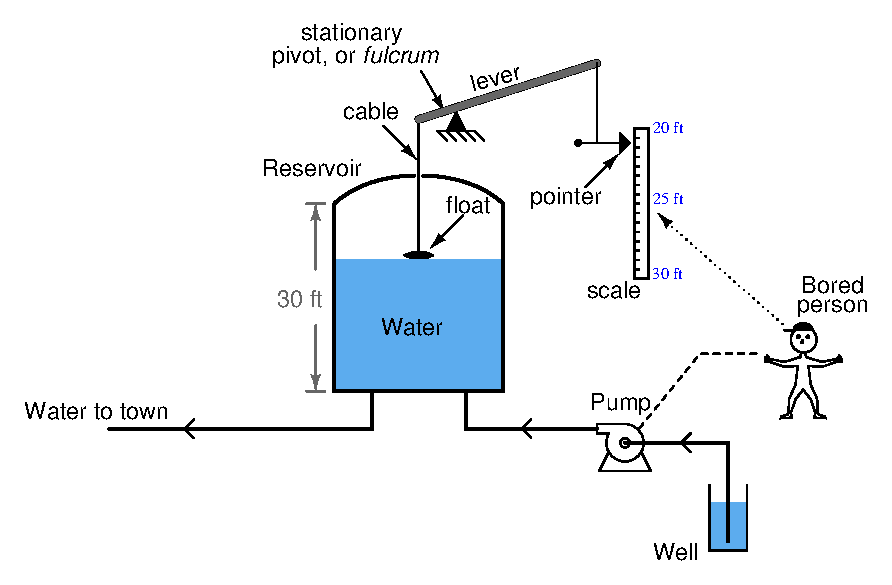
\includegraphics[width=15.5cm]{i00080x01.eps}$$

Sa grovt som det er, inneholder dette systemet {\it instrumentering}, og vi kan bruke standard instrumenteringstermer pa dets komponenter.  Bruk folgende termer pa dette vannforsyningssystemet, sa godt du kan:

\begin{itemize}
\item{} Prosess
\item{} Primart foleelement
\item{} Endelig reguleringsenhet
\item{} Maleomrade
\item{} Nedre omradeverdi (LRV)
\item{} Ovree omradeverdi (URV)
\item{} Målespenn
\item{} Indikator
\item{} Transmitter
\item{} Regulator
\item{} Malt variabel (eller prosessvariabel)
\item{} Kontrollert variabel (eller manipulert variabel)
\end{itemize}

\underbar{file i00080}
%(END_QUESTION)





%(BEGIN_ANSWER)

\begin{itemize}
\item{} Prosess: {\it vannet og alle tilhorende kar, ror og pumpe}
\item{} Primart foleelement: {\it flottor}
\item{} Endelig reguleringsenhet: {\it pumpe}
\item{} Maleomrade: {\it 20 fot til 30 fot}
\item{} Nedre omradeverdi (LRV): {\it 20 fot}
\item{} Ovree omradeverdi (URV): {\it 30 fot}
\item{} Målespenn: {\it 10 fot}
\item{} Indikator: {\it viser og skala}
\item{} Transmitter: {\it spak, pivot og kabler}
\item{} Regulator: {\it den kjedelige personen}
\item{} Malt variabel (eller prosessvariabel): {\it vannstand}
\item{} Kontrollert variabel (eller manipulert variabel): {\it pumpehastighet (pa/av-status)}
\end{itemize}

Skillet mellom maleomrade, LRV, URV og spenn er viktig.  Det vi maler her er vannstand i tanken mellom 20- og 30-fotsmerkene.  Differansen i niva mellom disse merkene er det vi kaller {\it spenn}.  Sa i dette tilfellet har vi et spenn pa 10 fot (30 fot $-$ 20 fot).  LRV er den nedre enden av maleomradet: 20 fot.  URV er den ovre enden av maleomradet: 30 fot.  {\it Omradet} for malingen omfatter bade LRV og URV, og oppgis ``20 til 30 fot''.

Pa samme mate, hvis du hadde en trykktransmitter i en luftseparasjonsprosess som var omradet fra 200 til 500 PSI, ville 200 PSI vare LRV, 500 PSI ville vare URV, og 300 PSI ville vare spennet.

\vskip 10pt

I et hvilket som helst instrumentsystem er {\it regulatoren} den som tar kontrollbeslutninger.  I dette tilfellet er det den kjedelige personen.  All annen maskinvare mellom flottoren og indikatoren overforer bare informasjon fra reservoaret til den kjedelige personen (regulatoren).

\vskip 10pt

For ordens skyld, jeg misliker virkelig termen ``kontrollert variabel''.  Jeg synes den er misvisende og forvirrende, men dessverre brukes den ofte nar man diskuterer prosessregulering.  Mens den ``malte'' eller ``prosess''-variabelen er det vi maler (og prover a holde pa setpunkt), er den ``kontrollerte'' eller ``manipulerte'' variabelen det vi justerer for a pavirke prosessvariabelen.  I dette tilfellet er prosessvariabelen vannstanden i reservoaret, og den kontrollerte (eller manipulerte) variabelen er pumpehastigheten.  Vi maler vannstand og kontrollerer den ved a sla pumpen pa og av.

Som en analogi, forestill deg et cruise-control-system i en bil.  Den malte (prosess-)variabelen er bilens hastighet, mens gasspedalposisjonen er den kontrollerte eller manipulerte variabelen, fordi pedalposisjonen er variabelen som justeres av cruise-control-systemet for a holde bilens hastighet pa setpunkt.

Her er noen generaliserte definisjoner:

\begin{itemize}
\item{} Malt variabel (eller prosessvariabel): {\it Variabelen vi maler, vanligvis med hensikt a holde den pa et konstant setpunkt}
\vskip 5pt
\item{} Kontrollert variabel (eller manipulert variabel): {\it Variabelen som direkte manipuleres av regulatoren, og som pavirker prosessvariabelen}
\end{itemize}


%(END_ANSWER)





%(BEGIN_NOTES)


%INDEX% Basics: water reservoir level control system
%INDEX% Process: municipal water storage tank

%(END_NOTES)


